%%%%%%%%%%%%%%%%%%%%%%%%%%%%%%%%%%%%%%%%%
% Short Sectioned Assignment LaTeX Template Version 1.0 (5/5/12)
% This template has been downloaded from: http://www.LaTeXTemplates.com
% Original author:  Frits Wenneker (http://www.howtotex.com)
% License: CC BY-NC-SA 3.0 (http://creativecommons.org/licenses/by-nc-sa/3.0/)
%%%%%%%%%%%%%%%%%%%%%%%%%%%%%%%%%%%%%%%%%

%----------------------------------------------------------------------------------------
%	PACKAGES AND OTHER DOCUMENT CONFIGURATIONS
%----------------------------------------------------------------------------------------

\documentclass[paper=a4, fontsize=11pt]{scrartcl} % A4 paper and 11pt font size

% ---- Entrada y salida de texto -----

\usepackage[T1]{fontenc} % Use 8-bit encoding that has 256 glyphs
\usepackage[utf8]{inputenc}
%\usepackage{fourier} % Use the Adobe Utopia font for the document - comment this line to return to the LaTeX default

% ---- Idioma --------

\usepackage[spanish, es-tabla]{babel} % Selecciona el español para palabras introducidas automáticamente, p.ej. "septiembre" en la fecha y especifica que se use la palabra Tabla en vez de Cuadro

% NOTA: en caso de problema al compilar, compruebe que tiene el paquete: texlive-babel-spanish.noarch

% ---- Otros paquetes ----

\usepackage{amsmath,amsfonts,amsthm} % Math packages
\usepackage{graphics,graphicx,floatrow} %para incluir imágenes y notas en las imágenes
\usepackage{listings}

\usepackage{url}

%% Define a new 'leo' style for the package that will use a smaller font.
\makeatletter
\def\url@leostyle{%
	\@ifundefined{selectfont}{\def\UrlFont{\sf}}{\def\UrlFont{\small\ttfamily}}}
\makeatother
%% Now actually use the newly defined style.
\urlstyle{leo}
\setlength{\parindent}{12pt}

% Para hacer tablas comlejas
\usepackage{multirow}
\usepackage{threeparttable}

%\usepackage{sectsty} % Allows customizing section commands
%\allsectionsfont{\centering \normalfont\scshape} % Make all sections centered, the default font and small caps

\usepackage{fancyhdr} % Custom headers and footers
\pagestyle{fancyplain} % Makes all pages in the document conform to the custom headers and footers
\fancyhead{} % No page header - if you want one, create it in the same way as the footers below
\fancyfoot[L]{} % Empty left footer
\fancyfoot[C]{} % Empty center footer
\fancyfoot[R]{\thepage} % Page numbering for right footer
\renewcommand{\headrulewidth}{0pt} % Remove header underlines
\renewcommand{\footrulewidth}{0pt} % Remove footer underlines
\setlength{\headheight}{13.6pt} % Customize the height of the header

\numberwithin{equation}{section} % Number equations within sections (i.e. 1.1, 1.2, 2.1, 2.2 instead of 1, 2, 3, 4)
\numberwithin{figure}{section} % Number figures within sections (i.e. 1.1, 1.2, 2.1, 2.2 instead of 1, 2, 3, 4)
\numberwithin{table}{section} % Number tables within sections (i.e. 1.1, 1.2, 2.1, 2.2 instead of 1, 2, 3, 4)

\setlength\parindent{0pt} % Removes all indentation from paragraphs - comment this line for an assignment with lots of text

\newcommand{\horrule}[1]{\rule{\linewidth}{#1}} % Create horizontal rule command with 1 argument of height



\usepackage[utf8]{inputenc}
\usepackage[T1]{fontenc}
\usepackage[spanish]{babel}
\usepackage{times}

\usepackage{color}
\definecolor{gray97}{gray}{.97}
\definecolor{gray75}{gray}{.75}
\definecolor{gray45}{gray}{.45}

\usepackage{listings}
\lstset{ frame=Ltb,
	framerule=0pt,
	aboveskip=0.5cm,
	framextopmargin=3pt,
	framexbottommargin=3pt,
	framexleftmargin=0.4cm,
	framesep=0pt,
	rulesep=.4pt,
	backgroundcolor=\color{gray97},
	rulesepcolor=\color{black},
	%
	stringstyle=\ttfamily,
	showstringspaces = false,
	basicstyle=\small\ttfamily,
	commentstyle=\color{gray45},
	keywordstyle=\bfseries,
	%
	numbers=left,
	numbersep=15pt,
	numberstyle=\tiny,
	numberfirstline = false,
	breaklines=true,
}

% minimizar fragmentado de listados
\lstnewenvironment{listing}[1][]
{\lstset{#1}\pagebreak[0]}{\pagebreak[0]}

\lstdefinestyle{consola}
{basicstyle=\scriptsize\bf\ttfamily,
	backgroundcolor=\color{gray75},
}

\lstdefinestyle{C}
{language=C,
}


\usepackage[pdftex,colorlinks=true,linkcolor=negro,urlcolor=blue]{hyperref,xcolor}
\definecolor{negro}{rgb}{0,0,0}

\graphicspath{ {./imagenes/} }
\usepackage{subfig}
\hypersetup{citecolor=blue}

\title{	
\normalfont \normalsize 
\textsc{{\bf Ingeniería de Servidores (2014-2015)} \\ Grado en Ingeniería Informática \\ Universidad de Granada} \\ [25pt]
\horrule{0.5pt} \\[0.4cm] % Thin top horizontal rule
\huge Memoria Práctica 4 \\ % The assignment title
\horrule{2pt} \\[0.5cm] % Thick bottom horizontal rule
}

\author{Jose Antonio Jiménez Montañés}

\date{\normalsize\today}

%----------------------------------------------------------------------------------------
% DOCUMENTO
%----------------------------------------------------------------------------------------
%
%\begin{figure}[H]
%	\centering
%	\includegraphics[width=0.5\textwidth]{gull}
%	\caption{Texto Prueba}
%	\label{fig:ddd}
%\end{figure}


%\cite{p1}


\begin{document}

\maketitle % Muestra el Título

\newpage %inserta un salto de página

\tableofcontents % para generar el índice de contenidos
\clearpage
\listoffigures

%\listoftables 

\newpage

%----------------------------------------------------------------------------------------
%	Cuestion 1
%----------------------------------------------------------------------------------------
\section{Instale la aplicación Phoronix. ¿Qué comando permite listar los benchmarks disponibles?}

Instalamos Phoronix:
\begin{figure}[H]
	\centering
	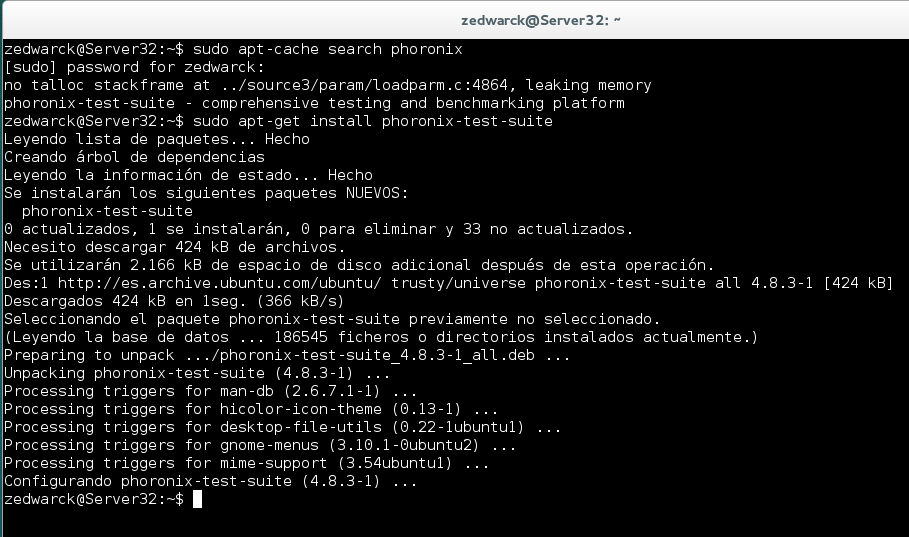
\includegraphics[width=1\textwidth]{p01f01}
	\caption{Proceso de instalación de Phoronix}
	\label{fig:p01f01}
\end{figure}

si ejecutamos phoronix-test-suite sin ningún modificador nos aparece una serie de modificadores disponibles en los cuales esta el que buscamos en nuestro caso: list-availables-tests

\begin{figure}[H]
	\centering
	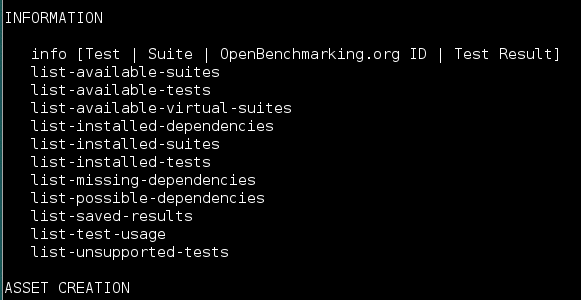
\includegraphics[width=0.8\textwidth]{p01f02}
	\caption{Visualización del comando buscado.}
	\label{fig:p01f02}
\end{figure}

Ejecutamos el comando: phoronix-test-suite list-availables-tests 

\begin{figure}[H]
	\centering
	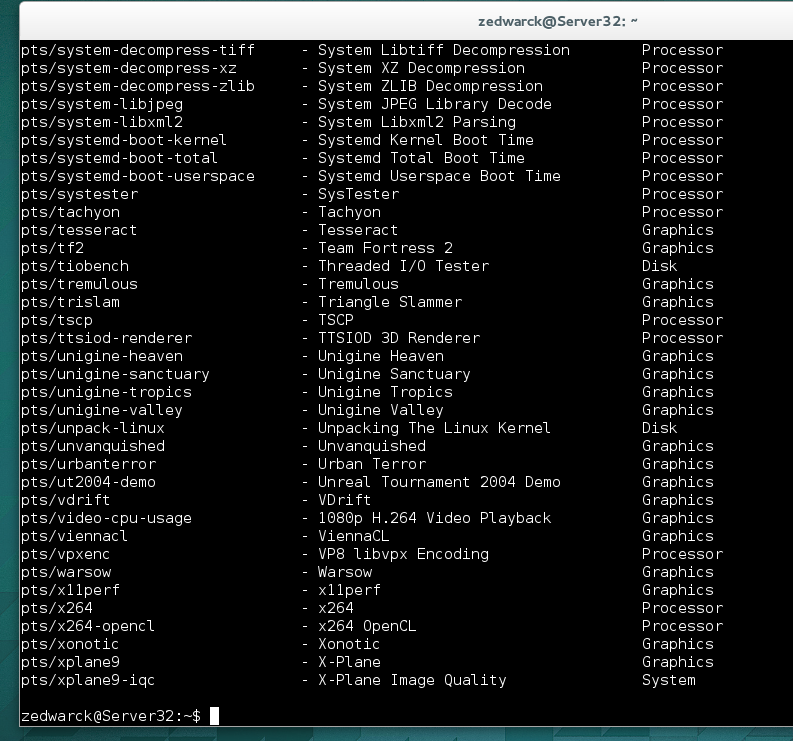
\includegraphics[width=1\textwidth]{p01f03}
	\caption{Lista de benchmarks disponibles}
	\label{fig:p01f03}
\end{figure}


\clearpage
%------------------------------------------------
% CUESTION OPCIONAL 1
%------------------------------------------------
\section{Seleccione, instale y ejecute uno, comente los	resultados.}

Hemos elegido un benchmark llamado "hdparm-read" que testea la velocidad de lectura de los dispositivos de almacenamiento. Incluso puede testear por dispositivos lógicos y no solo físicos.\\
Primero lo instalamos:
\begin{figure}[H]
	\centering
	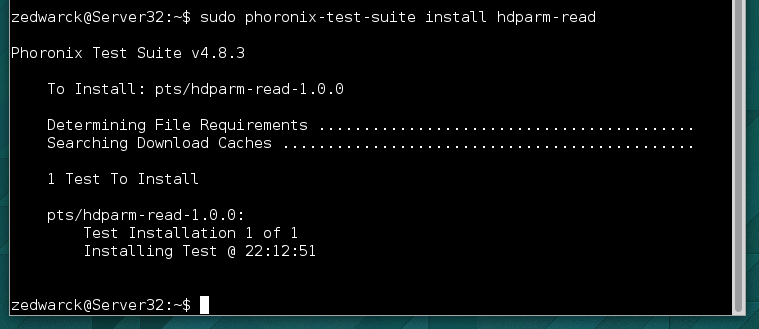
\includegraphics[width=1\textwidth]{po01f02}
	\caption{Instalacion del benchmark hdparm-read}
	\label{fig:po01f02}
\end{figure}


Luego lo ejecutamos:
\begin{figure}[H]
	\centering
	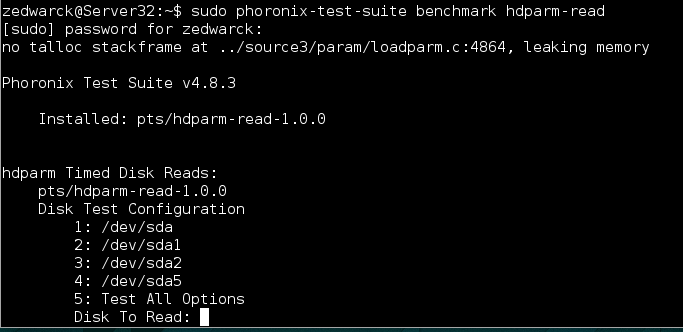
\includegraphics[width=1\textwidth]{po01f05}
	\caption{Ejecución del benchmark hdparm-read}
	\label{fig:po01f05}
\end{figure}

Después de elegir el sistema físico-lógico que queremos testear nos pregunta si queremos guardar los resultados del test(También nos muestra un resumen general del sistema).
\begin{figure}[H]
	\centering
	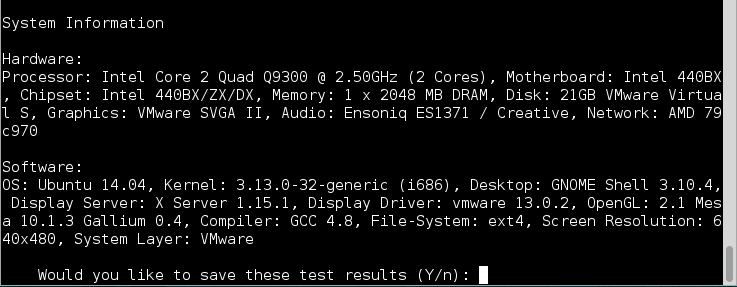
\includegraphics[width=1\textwidth]{po01f06}
	\caption{Resumen de nuestro sistema y confirmación de guardado de datos.}
	\label{fig:po01f06}
\end{figure}

El benchmark realiza cinco pasadas en nuestro caso:
\begin{figure}[H]
	\centering
	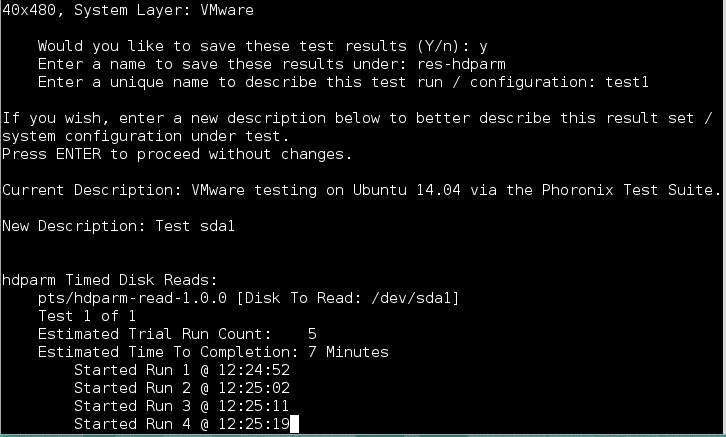
\includegraphics[width=1\textwidth]{po01f07}
	\caption{Realización de los test de disco.}
	\label{fig:po01f07}
\end{figure}

Finalmente nos muestra los resultados (Y nos pregunta si queremos visualizarlos en navegador.):
\begin{figure}[H]
	\centering
	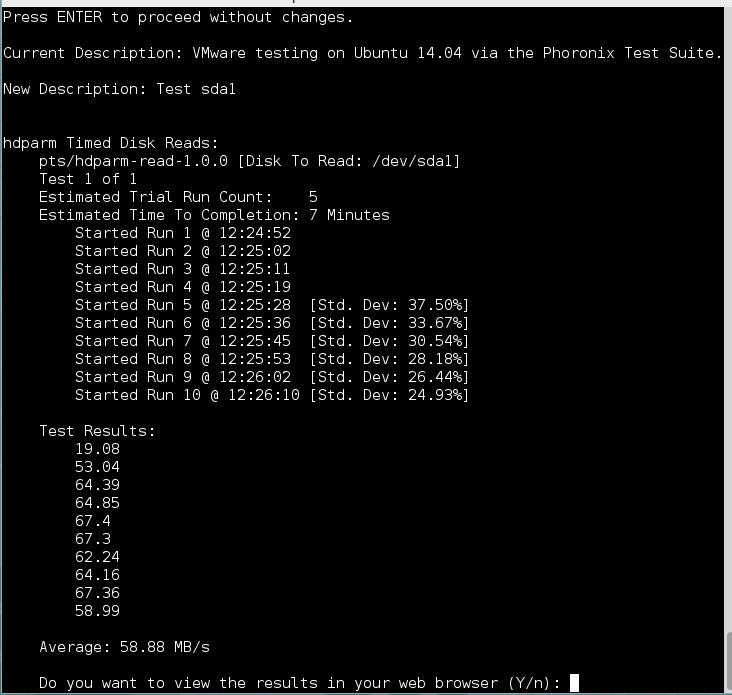
\includegraphics[width=0.65\textwidth]{po01f08}
	\caption{Resultado del benchmark hdparm-read.}
	\label{fig:po01f08}
\end{figure}

Resultados vistos en gráfica desde navegador.
\begin{figure}[H]
	\centering
	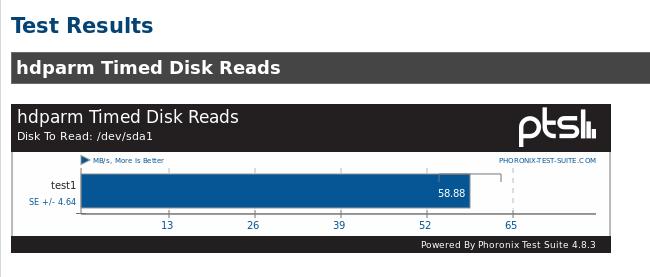
\includegraphics[width=0.6\textwidth]{po01f09}
	\caption{Resultado del benchmark hdparm-read en gráfica.}
	\label{fig:po01f09}
\end{figure}

%----------------------------------------------------------------------
% CUESTION 2	
%----------------------------------------------------------------------------------------
\section{En Apache Benchmark, de los parámetros que le podemos pasar al comando ¿Qué significa -c 30 ? ¿y -n 1000?}

La opción "-c 30" se refiere al numero de múltiples solicitudes para que puedan llevarse acabo a la vez, en este caso 30 solicitudes simultaneas.

La opción "-n 1000" indica el numero de solicitudes en una misma sesión de banchmarking, en nuestro caso en la misma sesión se realizarán 1000 solicitudes.


%-------------------------------------------------------------------------------------------
% CUESTION 3
%--------------------------------------------------------------------------------------------
\section{Ejecute ab contra a las tres máquinas virtuales (desde el SO anfitrión a las máquina virtuales de la red local) una a una (arrancadas por separado) y muestre las estadísticas. ¿Cuál es la que proporciona mejores 	resultados? Fíjese en el número de bytes transferidos, ¿es igual para cada máquina?}

Ejecutamos ab para:\\

1) Ubuntu Server x86:
\begin{figure}[H]
	\centering
	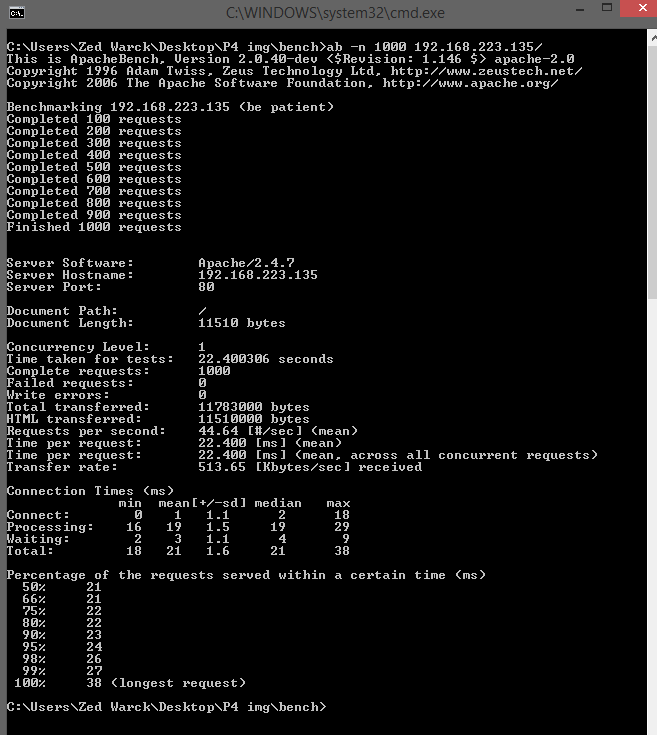
\includegraphics[width=0.8\textwidth]{p03f01}
	\caption{Ejecución y resultado de Apache Benchmark a un servidor Ubuntu Server x86.}
	\label{fig:p03f01}
\end{figure}

\clearpage
2) CentOS x64
\begin{figure}[H]
	\centering
	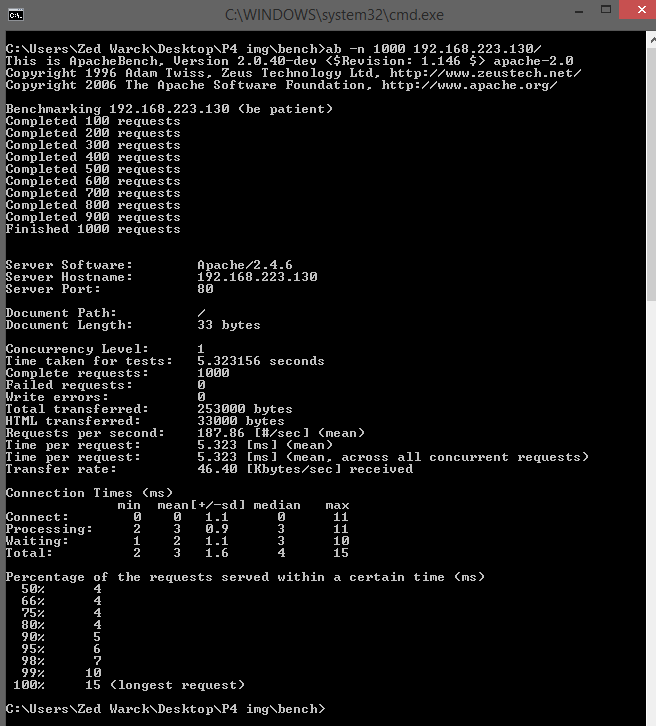
\includegraphics[width=1\textwidth]{p03f02}
	\caption{Ejecución y resultado de Apache Benchmark a un servidor CentOS x64.}
	\label{fig:p03f02}
\end{figure}

\clearpage
3) Windows Server 2008 R2
\begin{figure}[H]
	\centering
	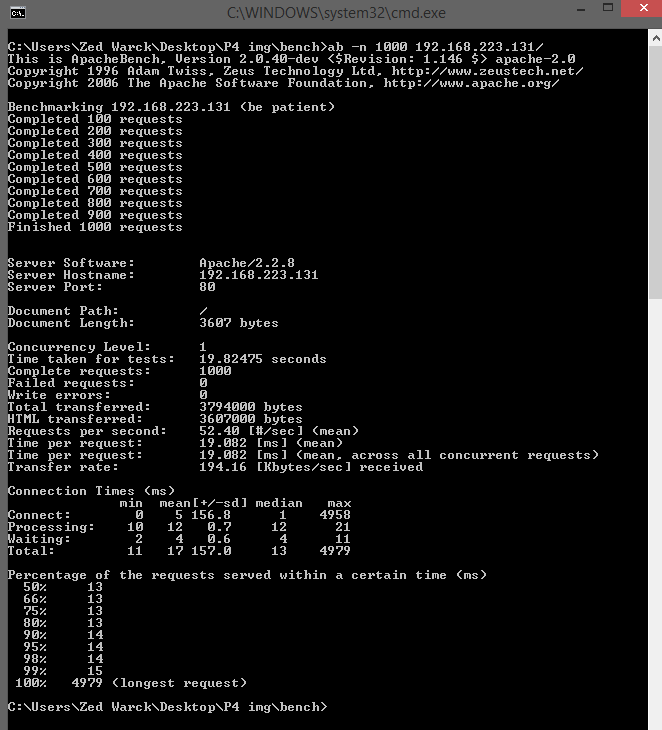
\includegraphics[width=1\textwidth]{p03f03}
	\caption{Ejecución y resultado de Apache Benchmark a un servidor Windows Server 2008 R2.}
	\label{fig:p03f03}
\end{figure}



Podemos observar como CentOS a resuelto las peticiones de una manera muchísimo más rápida que el resto de sistemas, así mismo también comprobamos como los bytes enviados difieren en cada una de las pruebas realizadas a los diferentes sistemas así como el tamaño de pagina siento CentOS el más eficiente en este aspecto.\\



%----------------------------------------------------------------------------------------
% CUESTION OPCIONAL 2:
%----------------------------------------------------------------------------------------
\section{¿Qué es Scala? Instale Gatling y pruebe los escenarios por defecto. \cite{c02o}}

Es un lenguaje de programación orientado a objetos. Se ejecuta en la máquina virtual de Java, por lo que puede integrarse con facilidad en los proyectos Java.\\

Para instalarlo en Ubuntu basta con: sudo apt-get install gatling\\






%----------------------------------------------------------------------------------------
% CUESTION OPCIONAL 3
%----------------------------------------------------------------------------------------
\section{Lea el artículo sobre Jmeter y elabore un breve resumen.}
El documento pretende comparar JMeter con Gatling, en la comparación tomas diversas medidas en un mismo caso simulado con 10000 usuarios y 30000 peticiones por minuto sobre un servidor web nginx.\\

Después de tomar las medidas hacen una valoración y se llega a la conclusión de que ambos son muy parecidos respecto al rendimiento. Solo destacar el nivel de procesamiento de JMeter es mayor debido a que se ejecuta sobre una maquina virtual java y eso produce un mayor volumen de procesamiento y carga de memoria RAM del servidor.

\clearpage
%----------------------------------------------------------------------------------------
% CUESTION 4
%----------------------------------------------------------------------------------------
\section{Instale y siga el tutorial en http://jmeter.apache.org/usermanual/build-web-test-plan.html realizando capturas de pantalla y comentándolas. En vez de usar la web de jmeter, haga el experimento usando alguna de sus máquinas virtuales(Puede hacer una página sencilla, usar las páginas de phpmyadmin, instalar un CMS, etc.).}

Instalamos JMeter (para windows hay que ejecutar el jmeter.bat que se encuentra dentro del subdirectorio bin) y nos aparece al ejecutarlo:
\begin{figure}[H]
	\centering
	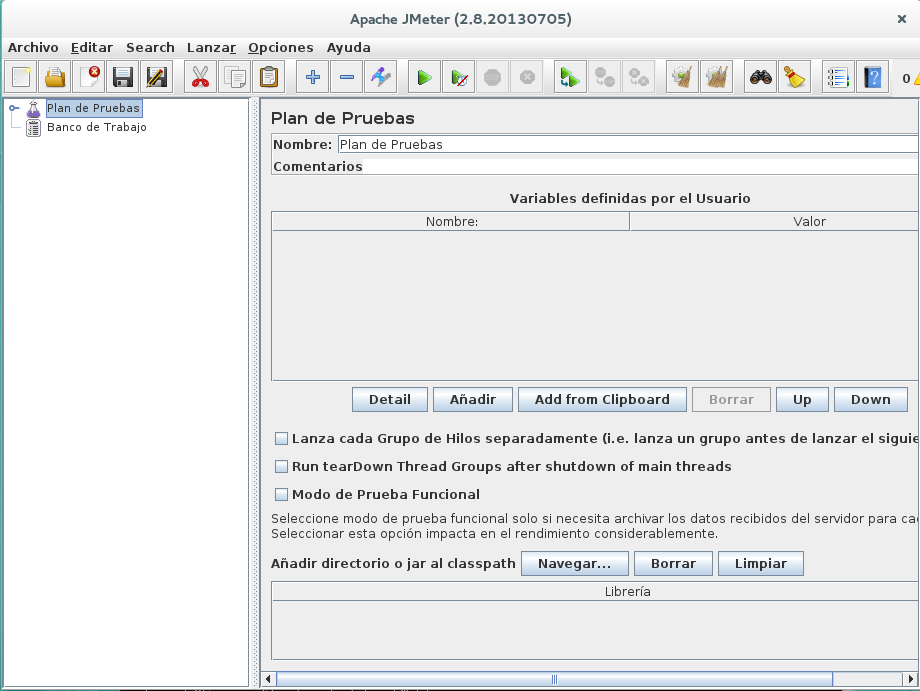
\includegraphics[width=1\textwidth]{p04f01}
	\caption{Ejecución de JMeter.}
	\label{fig:p04f01}
\end{figure}

\clearpage
Después creamos un grupo de hilos:

\begin{figure}[H]
	\centering
	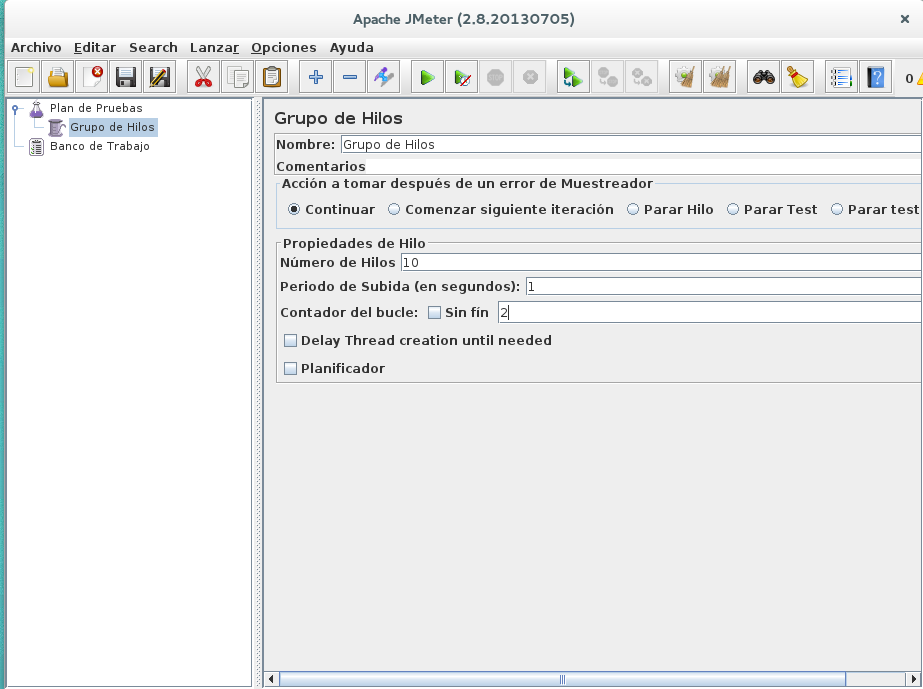
\includegraphics[width=1\textwidth]{p04f02}
	\caption{Configurando grupo de Hilos JMeter.}
	\label{fig:p04f02}
\end{figure}
\clearpage
En el siguiente paso configuramos los valores por defecto de las peticiones HTTP. Aquí configuramos la IP de nuestro servidor en la maquina virtual.
\begin{figure}[H]
	\centering
	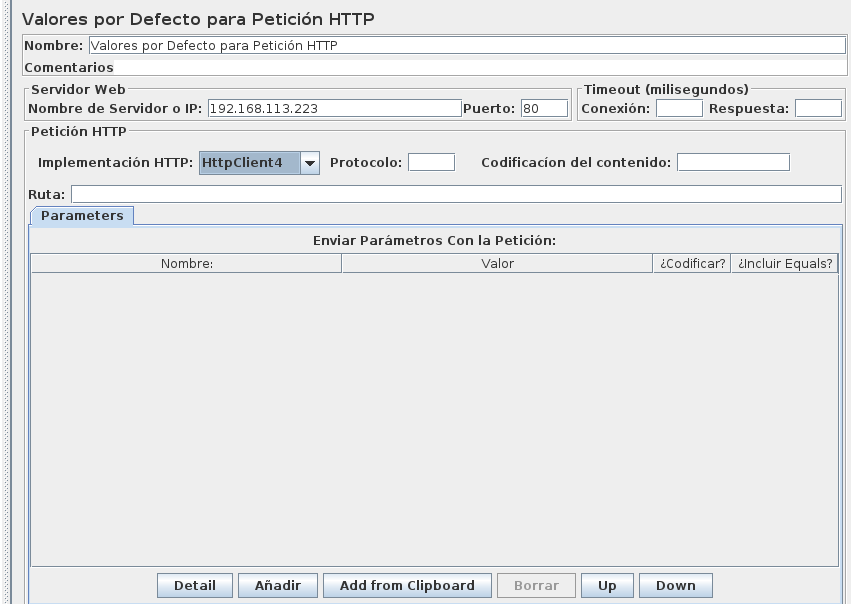
\includegraphics[width=1\textwidth]{p04f03}
	\caption{Configurando peticiones HTTP en JMeter.}
	\label{fig:p04f03}
\end{figure}
\clearpage
Luego incluimos los valores de cada peticion HTTP. Aquí es donde configuramos la ruta de acceso y archivo a ejecutar:
\begin{figure}[H]
	\centering
	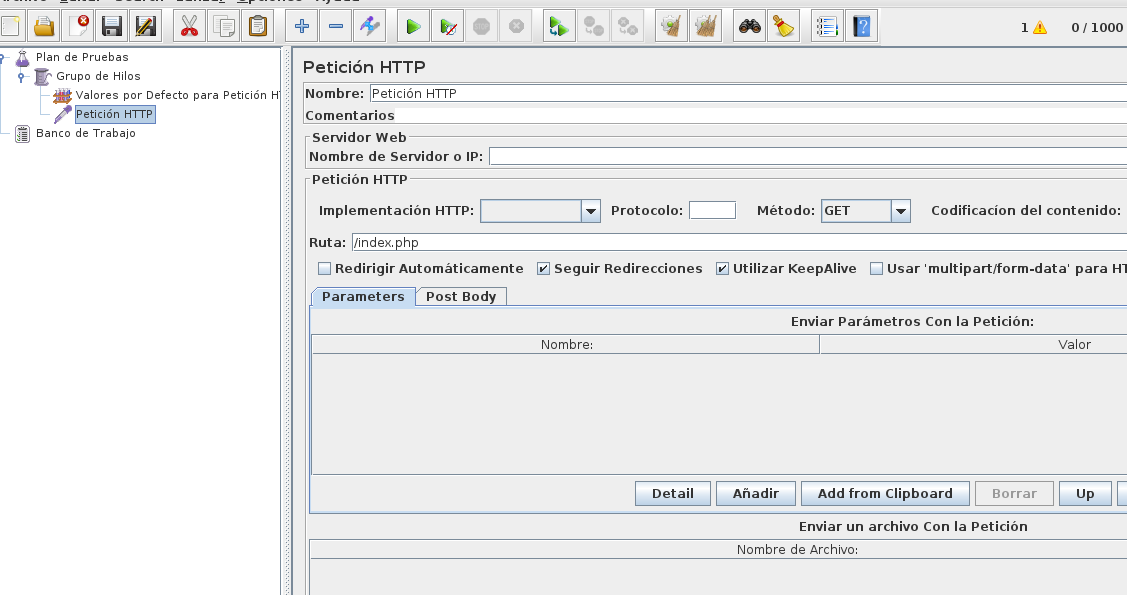
\includegraphics[width=1\textwidth]{p04f04}
	\caption{Configurando ruta de acceso de las peticiones.}
	\label{fig:p04f04}
\end{figure}
\clearpage
Finalmente se configura un listener para recopilar los datos. En nuestro caso vamos a hacerlo para que nos cree una gráfica al mismo tiempo:
\begin{figure}[H]
	\centering
	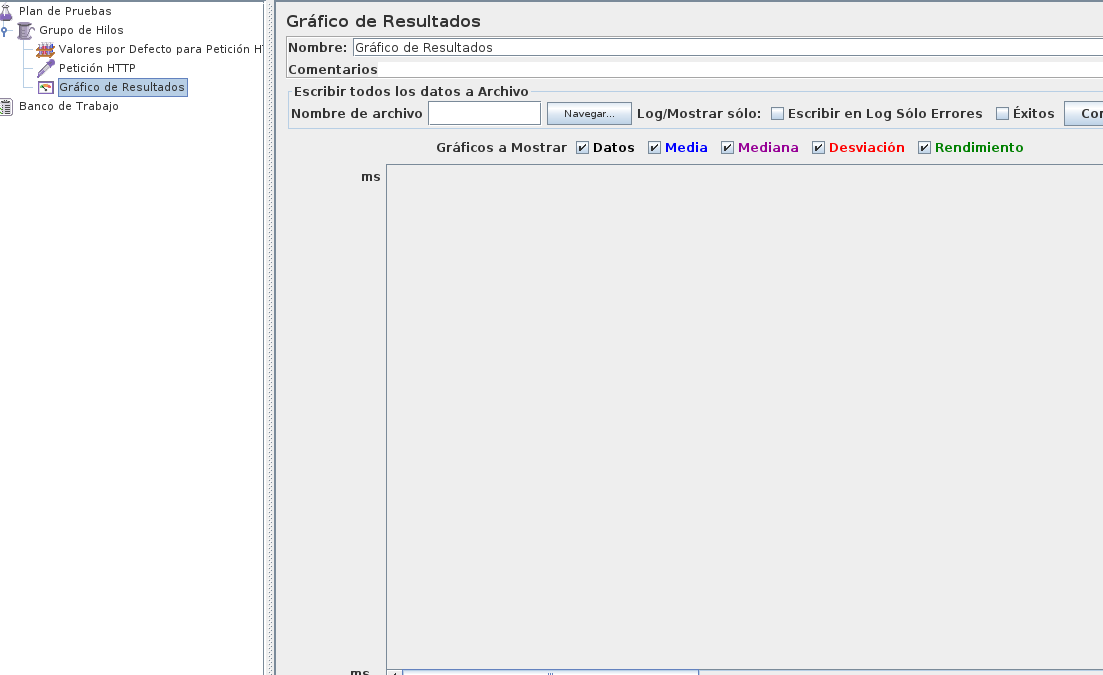
\includegraphics[width=1\textwidth]{p04f05}
	\caption{Configurando gráfica de resultados JMeter.}
	\label{fig:p04f05}
\end{figure}
\clearpage
Para finalizar, se ejecuta y se lanzan las peticiones (nuestro caso 1000 hilos).
\begin{figure}[H]
	\centering
	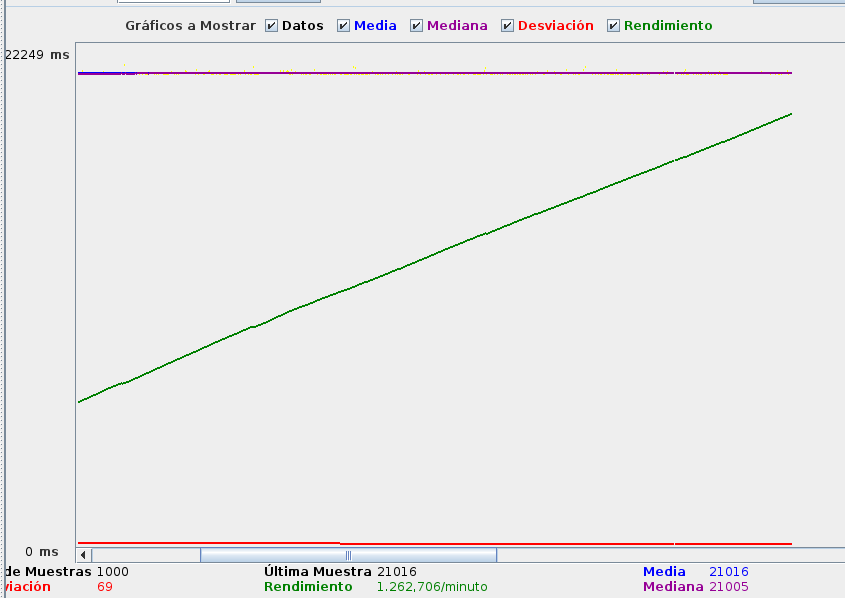
\includegraphics[width=1\textwidth]{p04f06}
	\caption{Resultados obtenidos en modo gráfica.}
	\label{fig:p04f06}
\end{figure}

\clearpage
%----------------------------------------------------------------------------------------
% CUESTION OPCIONAL 4
%----------------------------------------------------------------------------------------
\section{Seleccione un benchmark entre SisoftSandra y Aida.	Ejecútelo y muestre capturas de pantalla comentando los resultados.}

Después de instalarlo lo ejecutamos y tenemos:
\begin{figure}[H]
	\centering
	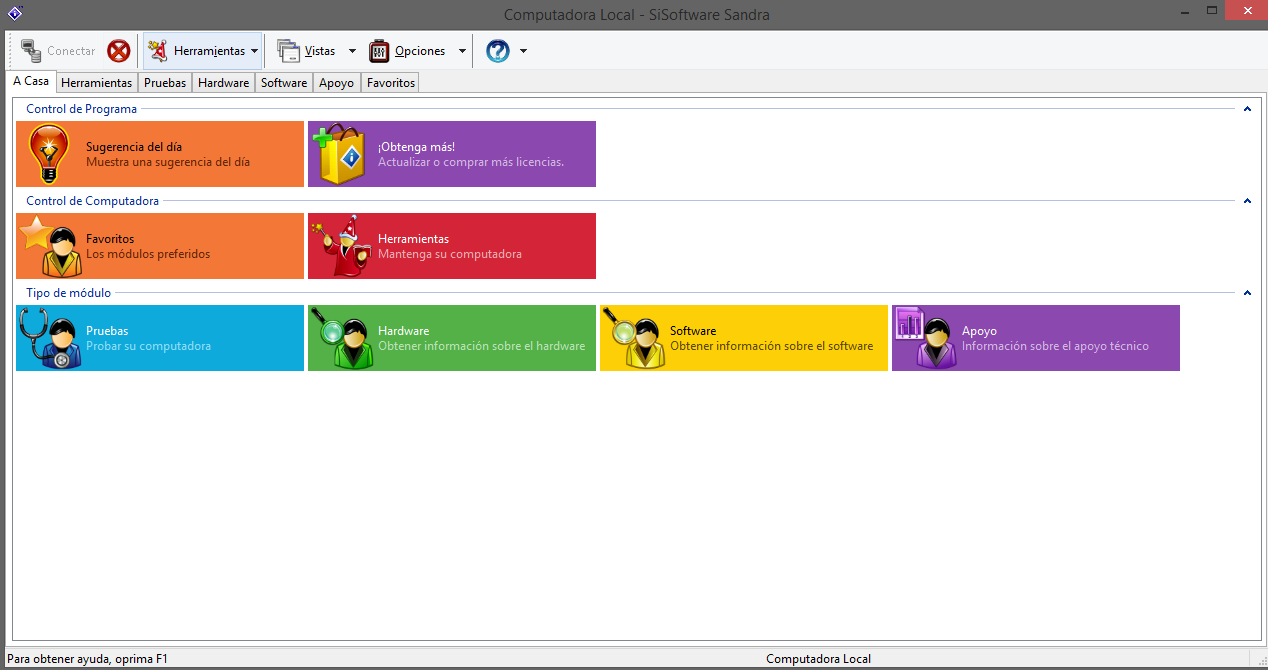
\includegraphics[width=0.8\textwidth]{po04f01}
	\caption{Pantalla inicial de SisoftSandra.}
	\label{fig:po04f01}
\end{figure}

Al darle a pruebas para testear nos muestra muchos tipos de tests que puede hacer a nuestra maquina. En nuestro caso elegimos que nos haga un benchmarking de la CPU y sus Gigaflops:

\begin{figure}[H]
	\centering
	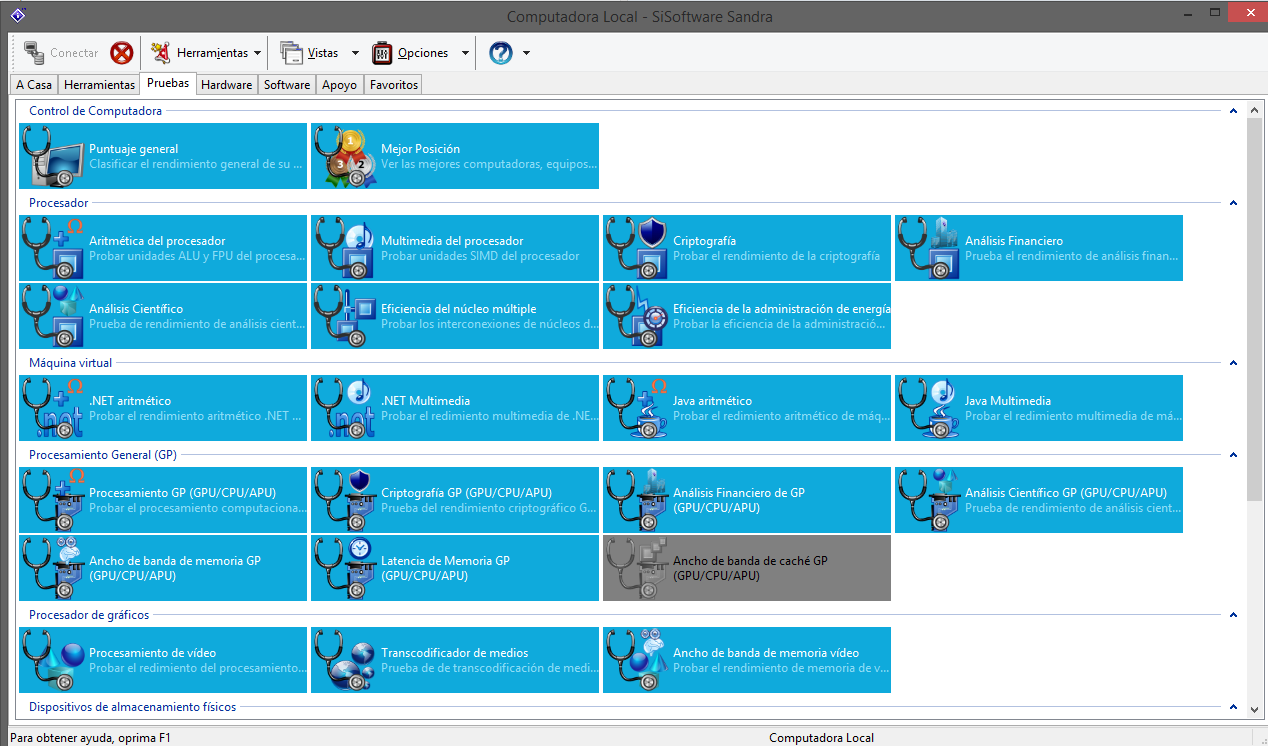
\includegraphics[width=0.7\textwidth]{po04f02}
	\caption{Diversos test de SisoftSandra.}
	\label{fig:po04f02}
\end{figure}

\clearpage
Después de un periodo de tiempo y una vez completado el test nos muestra el resumen y una grafica en la que podemos comparar con otros procesadores del mercado pudiendo elegir nosotros cuales son los procesadores de referencia:

\begin{figure}[H]
	\centering
	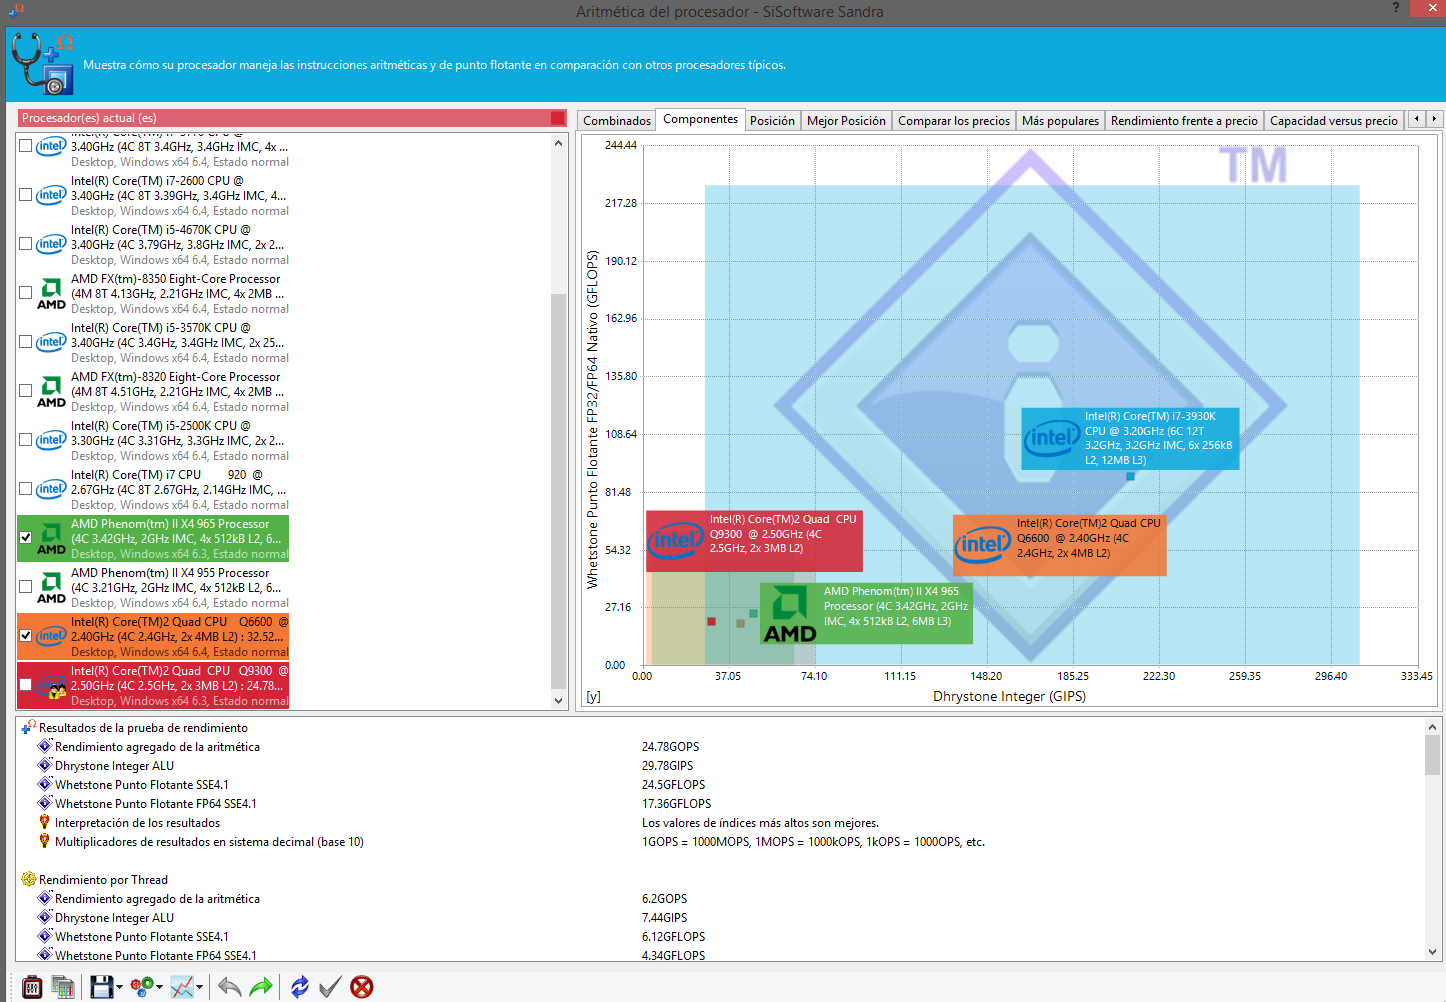
\includegraphics[width=1\textwidth]{po04f03}
	\caption{Resultado de testear la CPU con SiSoftSandra.}
	\label{fig:po04f03}
\end{figure}


\clearpage
%----------------------------------------------------------------------------------------
% CUESTION 5
%----------------------------------------------------------------------------------------
\section{Programe un benchmark usando el lenguaje que desee}

He programado un benchmark en c++ que testea la velocidad de lectura y escritura en disco.

\begin{lstlisting}[style=C]
#include <iostream>
#include <fstream>
#include <cstdlib>
#include <ctime>
#include <math.h>

using namespace std;

int main(int argc, char **argv){

	clock_t tiempo_ini, tiempo_fin;
	srand(time(NULL));

	int num_bloques = 100;
	int tam_bloque = 100; //(en MB)
	int i;

	cout << endl << "Benchmark HDD (by Zed Warck)" << endl;

	double tiempo_lectura = 0, tiempo_escritura = 0;
	int elementos=(tam_bloque*pow(2,20))/sizeof(int);
	int *bloque = new int[elementos];

	cout << endl << "Iniciando Benchmark HDD..." << endl;


	cout << endl << "Test de Escritura..." << endl;
	ofstream salida("test.dat", ios::out|ios::binary);
	for(i=0; i<num_bloques; i++){
		for(unsigned j=0; j<sizeof(elementos); j++)
			bloque[j] = rand()%static_cast<int>(pow(2,32));
		tiempo_ini = clock();
		salida.write(reinterpret_cast<const char*>(bloque), elementos*sizeof(int));
		tiempo_fin = clock();
		tiempo_escritura += static_cast<double>(tiempo_fin-tiempo_ini) / CLOCKS_PER_SEC;
	}
	cout << endl << "Tiempo de Escritura en HDD: " << tiempo_escritura << " segundos" << endl;
	
	
	cout << endl << "Test Lectura..." << endl;
	ifstream entrada("test.dat", ios::in|ios::binary);
	tiempo_ini = clock();
	for(i=0; i<num_bloques; i++)
		entrada.read(reinterpret_cast<char*>(bloque),elementos*sizeof(int));
	tiempo_fin = clock();
	tiempo_lectura = static_cast<double>(tiempo_fin - tiempo_ini) / CLOCKS_PER_SEC;
	cout << endl << "Tiempo de lectura en HDD: " << tiempo_lectura << " segundos" << endl;
	
	entrada.close();
	salida.close();
	if(remove("test.dat")!=0)
	perror("Error borrando ficheros temporales.");
	
	cout.precision(3);
	cout.setf(ios::fixed);
	cout.setf(ios::showpoint);

	cout << endl << "Tiempo total del test HDD: " << tiempo_escritura + tiempo_lectura << " segundos" << endl;
	
	float velocidad_r = num_bloques*tam_bloque / tiempo_lectura;
	float velocidad_w = num_bloques*tam_bloque / tiempo_escritura;
	
	cout << endl << "Velocidad de Lectura: " << velocidad_r << " MB/s" << endl;
	cout << endl << "Velocidad de Escritura: " << velocidad_w << " MB/s" << endl;
	return 0;
}


\end{lstlisting}

\clearpage
\bibliography{citas} %archivo citas.bib que contiene las entradas 
\bibliographystyle{unsrt} % hay varias formas de citar


\end{document}